We have seen that $\underline{u_i} = \frac{A\underline{v_i}}{\sigma_i}$ but, what happen if $\sigma_i = 0$?\\
Until now we have assumed that could not happen. Let's 2 examples, in the first we have the standard case while in the second is explained how to manage the case $\sigma_i = 0$.\\

\textbf{Example 1}
\[
A = \begin{bmatrix}
    4 & 4\\
    -3 & 3\\
\end{bmatrix} \hspace{1cm} \text{rank}(A) = 2
\]
We build two new matrices $X$ and $Y$:
\[
X = A^\intercal A = \begin{bmatrix}
    25 & 7\\
    7 & 25\\
\end{bmatrix} \hspace{1cm} \text{eigs}(X) = 
\begin{cases}
    \lambda_1 = 18 \hspace{1cm} \underline{v_1} = \begin{bmatrix}
        -\frac{\sqrt{2}}{2}\\
        \frac{\sqrt{2}}{2}\\
    \end{bmatrix}\\
    \lambda_2 = 32 \hspace{1cm} \underline{v_2} = \begin{bmatrix}
        \frac{\sqrt{2}}{2}\\
        \frac{\sqrt{2}}{2}\\
    \end{bmatrix}\\
\end{cases}    
\]
\[
Y = AA^\intercal = \begin{bmatrix}
    32 & 0\\
    0 & 18\\
\end{bmatrix} \hspace{1cm} \text{eigs}(Y) =
\begin{cases}
    \lambda_1 = 18 \hspace{1cm} \underline{u_1} = \begin{bmatrix}
        1\\
        0\\
    \end{bmatrix}\\
    \lambda_2 = 32 \hspace{1cm} \underline{u_2} = \begin{bmatrix}
        0\\
        1\\
    \end{bmatrix}\\
\end{cases}    
\]
So we have all elements for contructing the SVD:
\[
U = 
\begin{bmatrix}
    0 & 1\\
    1 & 0\\
\end{bmatrix}
\hspace{1cm}
\Sigma =
\begin{bmatrix}
    \sqrt{18} & 0\\
    0 & \sqrt{32}\\
\end{bmatrix}    
\hspace{1cm}
V =
\begin{bmatrix}
    -\frac{\sqrt{2}}{2} & \frac{\sqrt{2}}{2}\\
    \frac{\sqrt{2}}{2} & \frac{\sqrt{2}}{2}\\
\end{bmatrix}
\]
It is easy to verify that $A = U\Sigma V^\intercal$.

\textbf{Example 2}
\[
A = \begin{bmatrix}
    4 & 3\\
    8 & 6\\
\end{bmatrix}
\hspace{1cm}
\text{rank}(A) = 1    
\]\\
As in the example before, we start building our matrices $X$ and $Y$:
\[
X = A^\intercal A = \begin{bmatrix}
    80 & 60\\
    60 & 45\\
\end{bmatrix}
\hspace{1cm}
\text{eigs}(X) =
\begin{cases}
    \lambda_1 = 125 \hspace{1cm} \underline{v_1} = \begin{bmatrix}
        \frac{-4}{5}\\
        \frac{-3}{5}\\
    \end{bmatrix}\\
    \lambda_2 = 0 \hspace{1cm} \underline{v_2} = ?
\end{cases}
\]
How can we compute the value of $\underline{v_2}$? The idea is to bild a vector $\underline{v_2}$ such that it is orthogonal to $\underline{v_1}$. 
A possible solution is: $\underline{v_2} = \begin{bmatrix}
    \frac{3}{5}\\
    \frac{-4}{5}\\
\end{bmatrix}$.\\
The equation at the beginning of this page (the one regarding $\underline{u_i}$) can still be computed for the vector $\underline{v_1}$ in this case:
\[
\underline{u_1} = \dfrac{A\underline{v_1}}{\sigma_1} = \dfrac{1}{\sqrt{125}}\begin{bmatrix}
    4 & 3\\
    8 & 6\\
\end{bmatrix}
\begin{bmatrix}
    \frac{-4}{5}\\
    \frac{-3}{5}\\
\end{bmatrix} = \dfrac{1}{\sqrt{125}}\begin{bmatrix}
-5\\
-10\\    
\end{bmatrix}
\]
Now, the problem rises again because $\sigma_2 = 0$ so we cannot compute $\underline{u_2}$. In reality, we do not need to compute $\underline{u_2}$ because $\underline{u_1}$ and $\underline{v_1}$ are sufficient to recover the original matrix through (reduced) SVD, indeed:
\[
\underbrace{
\dfrac{1}{\sqrt{125}} \begin{bmatrix}
    -5 \\
    -10\\
\end{bmatrix}}_{U}
\underbrace{
\begin{bmatrix}
    \sqrt{125}
\end{bmatrix}}_{\Sigma}
\underbrace{ 
\begin{bmatrix}
    \frac{-4}{5} & \frac{-3}{5}\\
\end{bmatrix}}_{V}   
=
\begin{bmatrix}
    4 & 3\\
    8 & 6\\
\end{bmatrix}
\] 
We could have used also the full SVD with the following matrices:
\[
    U = \dfrac{1}{\sqrt{125}} \begin{bmatrix}
        -5 & -10\\
        -10 & 5\\
    \end{bmatrix}
\hspace{1cm}
\Sigma = \begin{bmatrix}
    \sqrt{125} & 0\\
    0 & 0\\
\end{bmatrix}
\hspace{1cm}
V = \begin{bmatrix}
    \frac{-4}{5} & \frac{-3}{5}\\
    \frac{-3}{5} & \frac{4}{5}\\
\end{bmatrix}
\]
Where $\underline{u_2}$ is the second column of the matrix $U$ and is a vector orthogonal to $\underline{u_1}$. All elements written here and not in the previous formulation are a waste of memory.
A concise recap of all versions of SVD:
\begin{enumerate}
    \item full SVD: $\underset{(m \times n)}{A} = \underset{(m \times m)}{U}\underset{(m \times n)}{\Sigma}\underset{(n \times n)}{V^\intercal}$
    \item economy SVD: $\underset{(m \times n)}{A} = \underset {(m \times n)}{U}\underset{(n \times n)}{\Sigma}\underset{(n \times n)}{V^\intercal}$
    \item reduced SVD: $\underset{(m \times n)}{A} = \underset{(m \times r)}{U}\underset{(r \times r)}{\Sigma}\underset{(r \times n)}{V^\intercal}$
    \item truncated SVD approximation: $\sum\limits_{i=1}^{\tilde{r}} \sigma_i\underline{u_i}\underline{v_i^\intercal}$
\end{enumerate}
For the first two cases the rank of $A$ is $n$, for the third is $r$ while in the first the approximation rank is decided.

\subsection{Geometrical interpretation of SVD}
Matrices $U, V^\intercal$ are orthonormal so, as mentioned in the section above, they represent a rotation (or reflection) while $\Sigma$, being a diagonal matrix, correspond to a scaling transformation. 
\begin{center}
    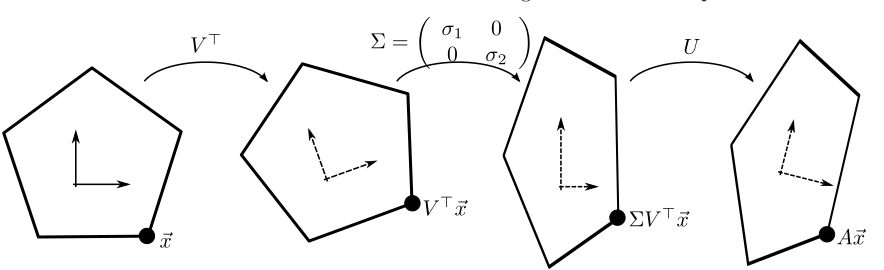
\includegraphics[scale=0.4]{../images/SVD_Geometric_Interpretation.png}
\end{center}
\textbf{Since for SVD no assumptions are made on the starting matrix, this means that \underline{any} matrix can be obtained from 2 rotations and 1 scaling.}\\

When $A$ is squared and symmetric ($A \in \mathbb{R}^{n\times n}, A=A^\intercal$)?

We can apply \textbf{polar decomposition}:
\[
A = QR    
\]
Where $Q$ is orthogonal and $S$ is symmetric positive semi-definite. Why? From SVD. 
\[
    A = U\Sigma V^\intercal = \underbrace{(UV^\intercal)}_{Q}\underbrace{(V\Sigma V^\intercal)}_{S}    
\]
In particular, the product of the two orthogonal matrices in the first parenthesis is always another orthogonal matrix. In this case of decomposition, matrix $A$ is obtained just by one rotation and one scaling (missing one more rotation with respect to classic SVD). Indeed, the second parenthesis results just in a stretch because $V$ and $V^intercal$ are two rotations identical and opposite, i.e. they cancels out. 

\subsubsection{Properties of SVD}
\begin{enumerate}[i]
    \item If A is orthogonal, then $\sigma_i = 1$ because if $A$ orthogonal then $A^\intercal A = I$
    \item All eigenvalues of a square matrix are $\leq \sigma_1$. Proof:
    \[
        ||A\underline{x}|| = ||U\Sigma V^\intercal \underline{x}|| = ||\Sigma V^\intercal \underline{x}|| \leq \sigma_1||V^\intercal \underline{x}|| = \sigma_1||\underline{x}|| \implies ||A\underline{x_i}|| \leq \sigma_1||\underline{x_i}||
    \]
    The matrix $U$ disappear becuase an orthogonal matrix, when multiplied, does not change the magnitude of a vector. If we consider
    \[
        ||A\underline{x_i}|| = ||\lambda_i\underline{x_i}|| = |\lambda_i|\cdot ||\underline{x_i}||
    \]
    \[
        |\lambda_i|\cdot ||\underline{x_i}|| \leq \sigma_1||\underline{x_i}|| \implies |\lambda_i| \leq \sigma_1 \hspace*{0.4cm} \forall i    
    \]
\end{enumerate}

\subsection{Snapshots method}
During real case scenarios, we will have a certain matrix $A \in \mathbb{m\times n}$ and it might happen that $m \gg n$ i.e. the number of samples is much greater than the number of features. In these cases, we can use the following trick to be more efficient.

For the SVD we need to compute both $AA^\intercal$ and $A^\intercal A$. Which one is better to start with? And why?
We would have $AA^\intercal: (m\times m)$ and $A^\intercal A: (n\times n)$. Given $m \gg n$ it is clear that the second one is better to start with becuase, being much smaller, it will be easier to computer its eigenvalues and eigenvectors.    


\subsection{Matrix norms}
This concept is an extension of the vector norm. Given a matrix $A \in \mathbb{R}^{m\times n}$, we define the matrix norm as:
\begin{itemize}
    \item \textbf{Frobenius norm}: $||A||_F = \sqrt{\sum\limits_{i=1}^{m}\sum\limits_{j=1}^{n}|a_{ij}|^2} = \sqrt{\Tr(A^\intercal A)} = \sqrt{\Tr(AA^\intercal)}$ \\
    Recall that $\Tr(AB) = \Tr(BA)$. \\
    Example:
    \[
        A = \begin{bmatrix}
            1 & 2\\
            3 & 4\\
            5 & 6\\
        \end{bmatrix} \hspace{1cm} ||A||_F = \sqrt{1^2 + 2^2 + 3^2 + 4^2 + 5^2 + 6^2} = \sqrt{91}
    \]
    \[
        \begin{bmatrix}
            1 & 2\\
            3 & 4\\
            5 & 6\\
        \end{bmatrix}
        \begin{bmatrix}
            1 & 3 & 5\\
            2 & 4 & 6\\
        \end{bmatrix} =
        \begin{bmatrix}
            1^2+2^2 & \hdots & \hdots\\
            \hdots & 3^2+4^2 & \hdots\\
            \hdots & \hdots & 5^2+6^2\\
        \end{bmatrix}  \implies \sqrt{\Tr(AA^\intercal)} = \sqrt{91}    
    \]
    If $U$ is orthogonal, what happen to $||AU||^2_F$?
    \[
        ||AU||^2_F = \Tr((AU)^\intercal AU) = \Tr(U^\intercal A^\intercal AU) = \Tr(A^\intercal A\underbrace{UU^\intercal}_{I}) = \Tr(A^\intercal A) = ||A||^2_F    
    \]
    This means that the Frobenius norm is invariant with respect to orthogonal transformations ($\dag$). \\ 
    The Frobenius norm is also equal to $\left(\sqrt{\sum\limits_{i=1}^{r}\sigma_i^2}\right)$ where $r$ is the rank of $A$. Proof:
    \[
        ||A||_F = ||U\Sigma V^\intercal||_F \overset{\dag}{=} ||\Sigma||_F \triangleq  \Tr\sqrt{(\Sigma\Sigma^\intercal)} = \sqrt{\sum\limits_{i=1}^{r}\sigma_i^2}    
    \]
    \item \textbf{P-norms}: Recall the p-norm for vectors:
    \[
        \underline{p} \in \mathbb{R}^n \implies ||\underline{p}||_p = \left(\sum\limits_{i=1}^n |p_i|^p\right)^{\frac{1}{p}}    
    \]
    Given $A \in \mathbb{R}^{m\times n}$ we can define the p-norm for that matrix as:
    \[
        ||A||_p = \underset{\underline{x} \in \mathbb{R}^n}{\sup} \dfrac{||A\underline{x}||_p}{||\underline{x}||_p} = \underset{\underline{x} \in \mathbb{R}^n, \hspace{0.1cm} ||\underline{x}||_p}{\sup} ||A\underline{x}||_p
    \]
    If you choose $p=2$ you get the operator norm and $||A||_2 = \sigma_1$.
\end{itemize}

\subsection{Eckart-Young theorem}
Having defined the norms, we can now proceed with the proof of the \textbf{Eckart-Young theorem} which states:\\

\emph{For either $||\cdot||_F$, $||\cdot||_2$ we have:}
\[
    ||A - A_k|| \leq ||A - B|| \hspace{1cm} \forall B \text{ of rank } k
\]
\emph{where} $A_k = \sum\limits_{i=1}^k \sigma_i\underline{u_i}\underline{v_i}^\intercal$ \emph{i.e. is the SVD approximation of rank k of the matrix A. Depending on the chosen norm you get:}
\[
    ||A - A_k|| = \begin{cases}
        \sigma_{k+1} \text{ if } ||\cdot||_2 \text{considered}\\
        \left(\sum\limits_{i=1}^{r} \sigma_i^2\right)^{\frac{1}{2}} \text{ if } ||\cdot||_F \text{ considered}
    \end{cases}
\]
There will be 2 proofs, one for each type of norm. 

\subsubsection{Proof considering $||\cdot||_F$}
We start from the \textbf{Weyl inequality}:
\[
    \sigma_{i+j-1}(X+Y) = \sigma_i(X) + \sigma_j(Y)    
\]
Where a generic $\sigma_k(E)$ is the k-eiths singular value of the matrix $E$.  
We define 
\[
X = A_k - B \hspace{2cm} Y = B    
\]
So we have
\[
\sigma_{i+k}(A) \leq \sigma_i(A-B) + \underbrace{\sigma_{k+1}(B)}_{0}
\]
The last component has value of 0 because the matrix $B$ has rank equal to $k$.
\[
||A - A_k||_F^2 = \left(\sum\limits_{i=k+1}^r \sigma_i^2(A)\right) \overset{\text{shift}}{\overset{\downarrow}{=}} \left(\sum\limits_{i=1}^{r-k} \sigma_{i+k}^2(A)\right) \leq \left(\sum\limits_{i=1}^{r-k} \sigma_{i+k}^2(A - B)\right) \leq \left(\sum\limits_{i=1}^{\min(m,n)} \sigma_{i+k}^2(A-B)\right) = ||A-B||_F^2
\]
In particular, recall that $A = \sum\limits_{i=1}^{r} \sigma_i\underline{u_i}\underline{v_i^\intercal}$ and $A_k = \sum\limits_{i=1}^{k} \sigma_i\underline{u_i}\underline{v_i^\intercal}$. The theorem is proved just by picking the first and last components of the inequality written above. 


